\section{Networks}\label{section:networks}

    In this section MultiResUNet and SegAN models are presented.
    Since U-Net architecture was considered as the baseline in this thesis, their advantages and their bootlenecks were shown through their trade-off in computation complexity and their detection performance.

    \subsection{MultiResUNet}\label{section:multiresunet}

        As discussed in Section~\ref{section:unet}, U-Net is a state-of-the-art neural network in medical imaging, but it has some drawbacks in certain conditions.
        Starting from this point, \citet{ibtehaz2020multiresunet} proposed a new U-Net variant, MultiResUNet including several modifications examined below.

        \begin{figure}
    \centerline{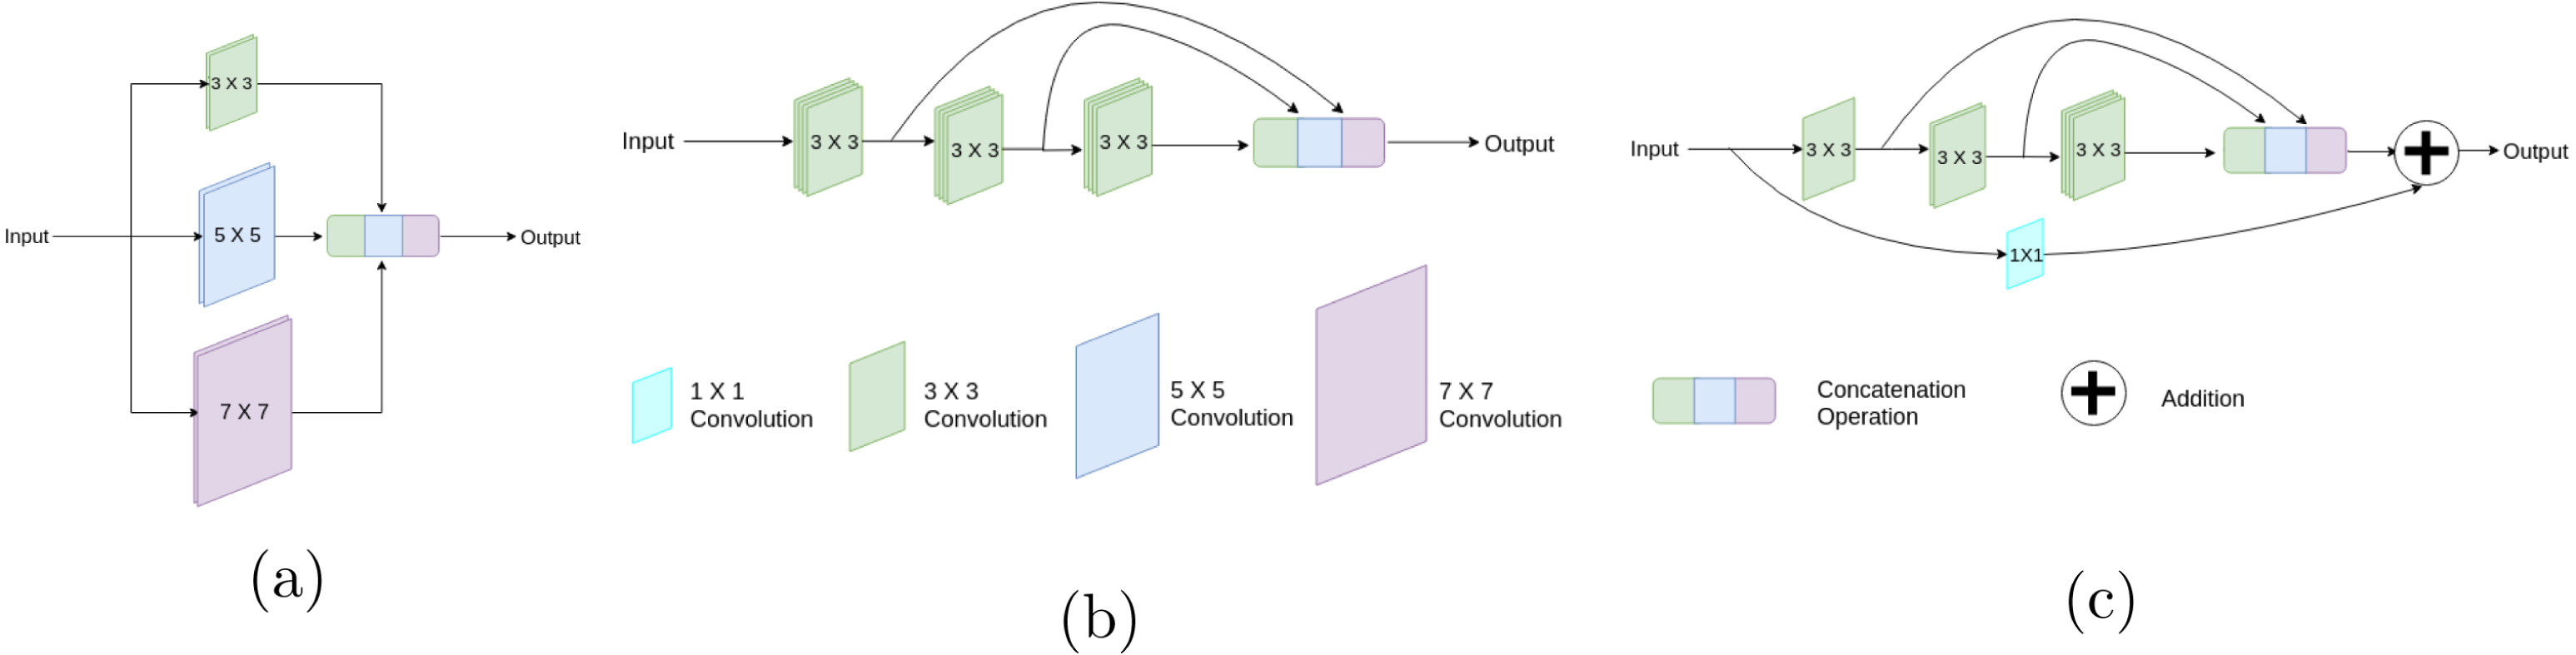
\includegraphics[width=1\columnwidth]{04-methodology/figures/multiresunet-multiresblock-steps.jpg}}
    \caption{Evalution of MultiRes block : \textbf{(a)} Inception-like block \textbf{(b)} a more expensive attempt \textbf{(c)} MultiRes block \cite{ibtehaz2020multiresunet}}
    \label{figure:multiresunet-multiresblock-steps}
\end{figure}

        Irregularity and images in different scales are common conditions in medical imaging samples.
        Neural networks aiming to get accurate results in medical imaging should be able to overcome these kind of problems.
        Images in different scales is an ongoing situation for medical imaging even if there are some studies about it, because of that, it is not possible to say that this issue has been definitely resolved.
        \citet{szegedy2015going} proposed Inception architecure built on convolutional layers with various kernel size to minimize the difference of the scales between images.
        MultiResUNet has an improvement similar to Inception architecture.
        In addition to the 3x3 convolution layer in the classic U-Net, MultiResUnet has convolution layers in different kernels such as 5x5 and 7x7.
        Figure~\ref{figure:multiresunet-multiresblock-steps} shows the evolution of the MultiRes blocks with different attempts, resulting from the different uses of these kernels.
        These multires blocks have replaced the sequences of two convolutional layer in the vanilla U-Net.

        \begin{figure}
    \centerline{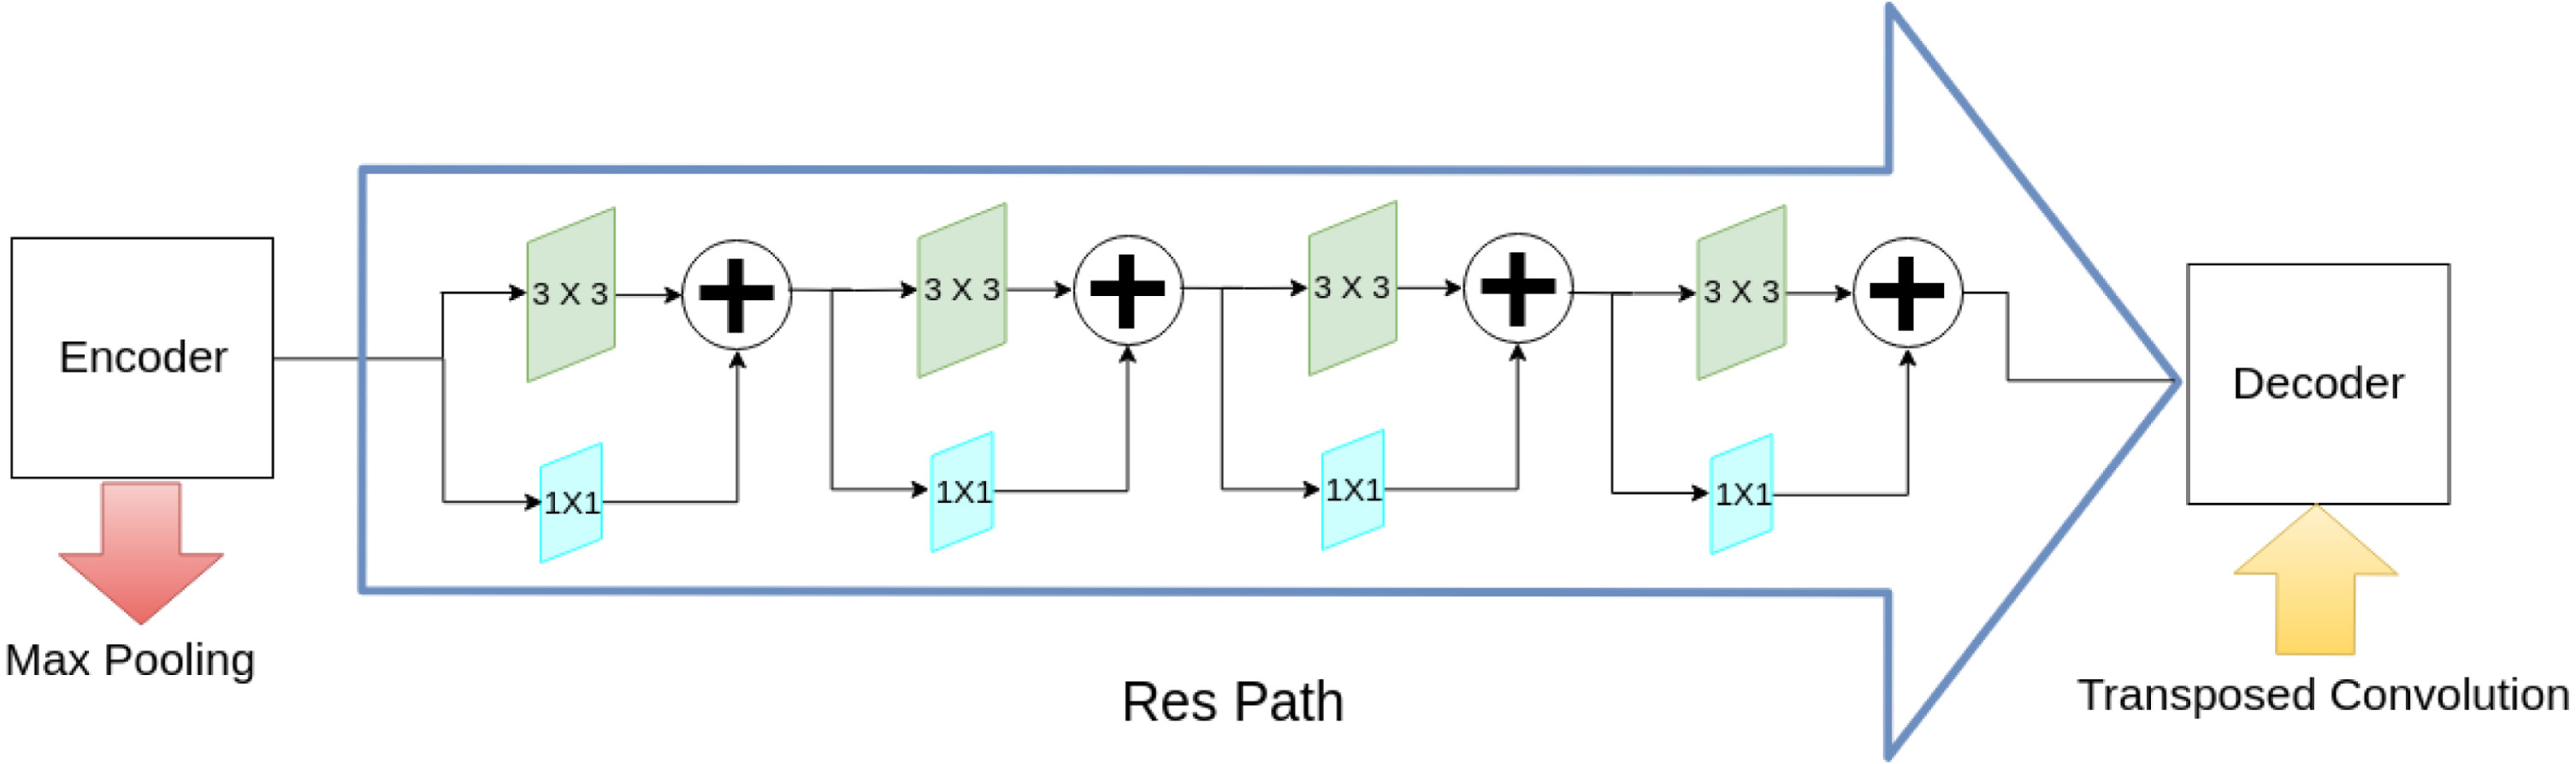
\includegraphics[width=1\columnwidth]{04-methodology/figures/multiresunet-respath.jpg}}
    \caption{Proposed Res path with residual connections \cite{ibtehaz2020multiresunet}}
    \label{fig:multiresunet-respath}
\end{figure}

        One of the significant improvement in U-Net is using the skip connections between the encoder and decoder.
        Thus, features which are lost during pooling are recovered and transferred from encoder block to decoder block.
        It is expected that the features sent by encoder to decoder are low level while the features in the decoder are expected to be high level.
        They thought that this may cause a semantic gap between the encoder and decoder and proposed another improvement called Res path which can be seen in Figure~\ref{figure:multiresunet-respath}.
        The proposed Res path consists of convolutional layers connected by residual connections to make learning easier \cite{drozdzal2016importance}.
        The features are being sent from encoder to decoder are transmitted over the Res paths instead of classical skip connections of U-Net.
        The proposed MultiResUNet framework is shown in Figure~\ref{figure:multiresunet-architecture} with the all improvements.

        \begin{figure}
    \centerline{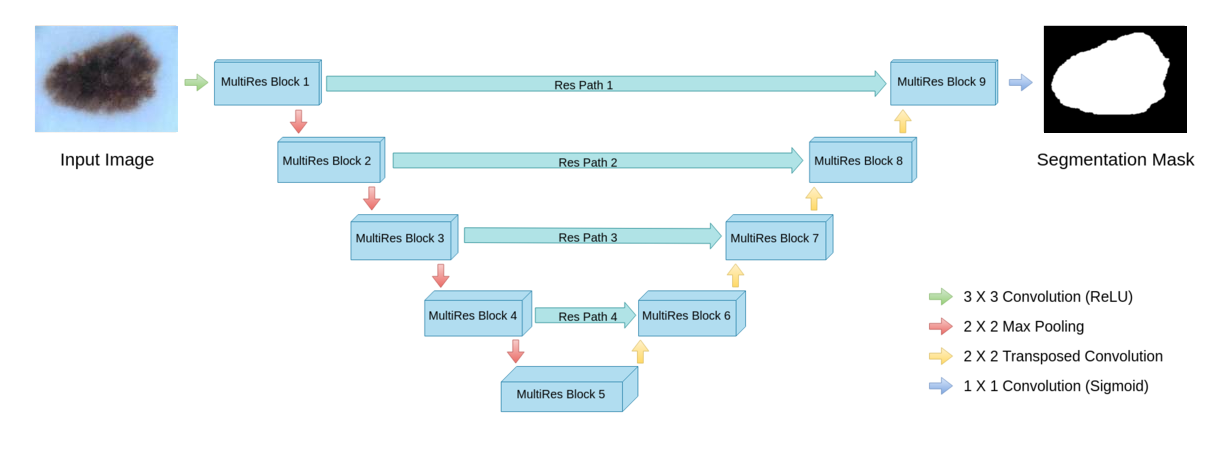
\includegraphics[width=1\columnwidth]{04-methodology/figures/multiresunet-architecture.png}}
    \caption{MultiResUnet architecture}
    \label{fig:multiresunet-architecture}
\end{figure}

        MultiResUNet has been tested and evaluated through several datasets including Murphy lab, ISBI 2012, ISIC 2018, CVC-ClinicDB, and BraTS17
        with different modalities such as fluorescence microscopy, electron microscopy, dermoscopy, endoscopy, and MRI respectively.
        Their results show that the MultiResUNet offers more accurate results than the classical U-Net for the all 5 different datasets especially in dermoscopy and endoscopy images.

    \subsection{SegAN}\label{section:segan}

        \citet{xue2018segan} proposed a new semantic segmentation network inspired by classical generative adversarial networks (GANs).
        Their motivation about proposing a GAN based segmentation network is that there was no such GAN based network that give accurate results.
        \citet{luc2016semantic} have tried to segment images with a GAN-like network but explained that the network is unstable for image segmentation tasks.
        The creators of SegAN claim that the single scalar input, which was created by the discriminator,  might the reason of the unstability in image segmentation of conventional GANs.
        Because semantic segmentation requires pixel-level mapping, and the discriminator network of GAN may not be able to produce sufficient gradient feedback with single scalar output.
        The differences of the proposed network for semantic segmentation compared to classical GAN ​​are mentioned below.

        SegAN consists of two networks segmentor and critic which can be seen in Figure ~\ref{figure:segan-architecture} similar to Generator and Discriminator networks of conventional GANs.
        It looks like a game as in GAN where the segmentor tries to fool the critic with the samples it creates.

        \begin{figure}
    \centerline{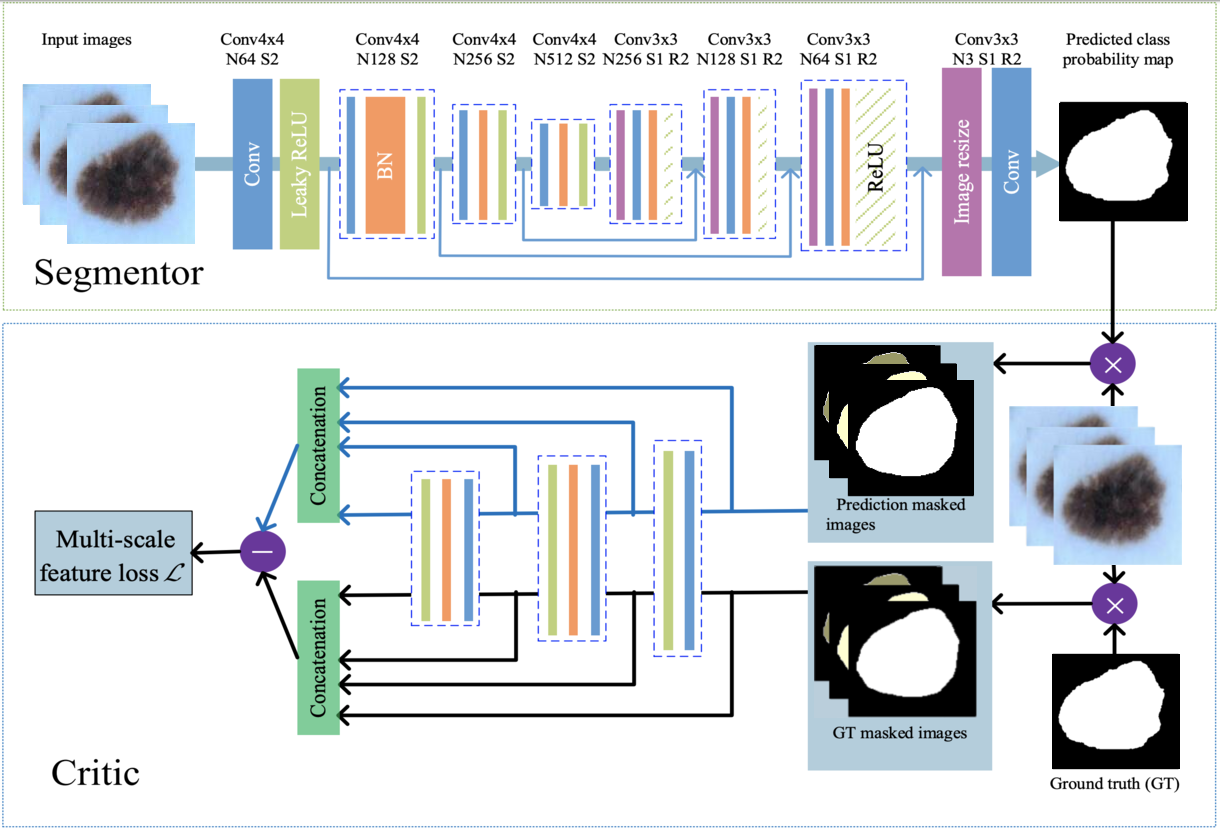
\includegraphics[width=1\columnwidth]{04-methodology/figures/segan-architecture.png}}
    \caption{SegAN architecture}
    \label{fig:segan-architecture}
\end{figure}

        The main difference arises with multi-scale loss function. While two separate loss functions are defined for generator and discriminator in GAN,
        segmentor and critic use a common multi-scale loss function to force the both networks of SegAN to learn local and global features which acquires relations between pixels.

        The critic network aims to maximize multi-scale loss function using the differences of CNN features between the predicted images and the ground truth.
        On the other hand, segmentor network, which is an FCN, tries to minimize the loss function used in the critic network.
        They claim that the SegAN can learn spatial pixel features with the help of the proposed multi-scale loss function even the images are in different scales.

        SegAN is trained with the BRATS 2015 dataset and achieved remarkable results compared to other state-of-the-art models, including U-Net, in the field of semantic segmentation.
